\documentclass{elteikthesis}

\usepackage{ucs}
\usepackage[utf8x]{inputenc}
\usepackage[T1]{fontenc}
\usepackage[english, hungarian]{babel}
\usepackage{hyperref}
\selectlanguage{hungarian}

\usepackage{listings}
\usepackage{color}

\definecolor{dkgreen}{rgb}{0, 0.6, 0}
\definecolor{grey}{rgb}{0.5, 0.5, 0.5}
\definecolor{mauve}{rgb}{0.58, 0, 0.82}

\lstset{
  frame = tb,
  language = xml,
  aboveskip = 3mm,
  belowskip = 3mm,
  showstringspaces = false,
  columns = flexible,
  basicstyle = {\small\ttfamily},
  numbers = none,
  numberstyle = \tiny\color{grey},
  keywordstyle = \color{blue},
  commentstyle = \color{dkgreen},
  stringstyle = \color{mauve},
  breaklines = true,
  breakatwhitespace = true,
  tabsize = 3
}

\usepackage[rightcaption]{sidecap}
 
\usepackage{graphicx} %package to manage images
\graphicspath{ {pics/} }

\title{\textbf{Integrált adatbázis-fejlesztői környezet SQL-hez}}
\author{Lestár Norbert}
\supervisor{dr Nikovits Tibor}
\supervisorstitle{Mestertanár}
\period{Programtervező informatikus BSc}
\thesisyear{2017}
\department{Információs Rendszerek Tanszék}

\begin{document}

\frontmatter

	\maketitle
	\tableofcontents
	
\mainmatter

\chapter{Bevezetés} 
Nem minden felhasználó ért az SQL-hez, részben ezért lehet szükség egy integrált fejlesztői
környezetre. A szintaxis kiemelésnek köszönhetően így könnyű észrevenni és javítani a hibákat,
valamint lényegesen gyorsabban meg lehet tanulni az SQL-t. Bizonyos műveleteket akár az SQL teljes
ismerete nélkül is elvégezhet bárki. Továbbá tapasztalt felhasználóknak is hasznos eszköz, mert
letisztult és átlátható felületet biztosít az adatbázis objektumainak megtekintésére. Ezen felül a
diagramok segítségével könnyen leolvashatóvá válnak az adatbázis különböző tulajdonságai, valamint
az egyedi, felhasználó által létrehozott táblák is.
A megvalósított program képes ezekre:
egy szerkesztőn lehetőség nyílik SQL, illetve PL/SQL kód leírására,
esetleg ha már van kész kód akkor annak betöltésére.
Oracle SQL adatbázishoz lehet csatlakozni, és
csatlakozás után a felhasználói felület segítségével különböző dolgokra nyílik lehetőség:
\begin{itemize}
  \item Adatbázisban megtalálható objektumok megtekintésére, törlésére, illetve újak létrehozására,
  \item program használata során kipróbált SQL, illetve PL/SQL parancsok mentésére,
  \item különböző diagramok (kördiagram, oszlopdiagram) megtekintésére lekérdezések segítségével,
  \item szintaxis kiemelésre (diagramokat létrehozó utasítás esetén is),
  \item valamint lekérdezési tervek megtekintésére is.
\end{itemize}
A programomat \textit{DiagramQuery} néven fogom a továbbiakban említeni.

\chapter{Felhasználói dokumentáció}
\textit{DiagramQuery} első sorban lehetőséget biztosít egy Oracle SQL adatbázishoz való kapcsolódásra.
A kapcsolatokat tartalmazó adatokat el is lehet menteni (illetve lehetőség van kézzel leírni,
ez kifejtésre kerül az első szekcióban.), illetve betölteni egy .xml formátumú fájlból.

A kapcsolat felépítése után lehetőség van egy szerkesztő ablakban SQL valamint PL/SQL parancsokat írni,
illetve diagramokat is itt lehet készíteni, ennek részletezése a 3. szekcióban történik meg.

\section{Telepítés és beállítás}
A \textit{DiagramQuery} telepítése történhet bármely operációs rendszeren amelyen rendelkezésre áll a
Clang 4.8 és a Qt 4.8-as verziója. A program ezeken lett tesztelve, természetesen működhet más verzióval is,
de nem garantált. Ezeken felül szükség van OCI 1.2-re is, és fordítani kell a megfelelő Qt-s plugint.
Illetve bizonyos linux disztribuciók alatt lehetőség van közvetlen letöltésre is.

Lehetőség van későbbi fejlesztések során további adatbázis-kezelők hozzáadására, ezekhez elég lesz a Clang, illetve Qt birtoklása.
Telepítés után lehetőség van manuálisan létrehozni kapcsolatokat. Ha ezt kívánja tenni hozzon létre egy
\textit{Connections} mappát a futtatható állomány mellé, és hozzon létre egy .xml kiterjesztésű fájlt a kívánt névvel.
A fájl felépítése a következő legyen:
\begin{itemize}
  \item Connection címkék között legyen elhelyezve az egész, illetve legyen a címkének egy attribútuma: name, a kapcsolat nevével,
  \item host címkék között a kapcsolat címe legyen,
  \item port címkék között legyen megadva a kapcsolat portja,
  \item service címkék között legyen a szervíz neve,
  \item illetve username címkék között a bejelentkezéshez szükséges felhasználónév.
\end{itemize}
Ha valamelyik mezőt nem szeretné eltárolni, akkor azt címkével együtt hagyja ki.
Egy konkrét példa a fájlra: (port megadása nélkül)

\begin{lstlisting}
  <?xml version="1.0" encoding="UTF-8"?>
  <Connection name="Elte">
      <host>aramis.inf.elte.hu</host>
      <service>eszakigrid97</service>
      <username>A8UZ7T</username>
  </Connection>
\end{lstlisting}

Miután létrehoztuk a fájlt el is kezdhetjük a program használatát, további beállításra nincs szükség.

\section{Kapcsolódás}
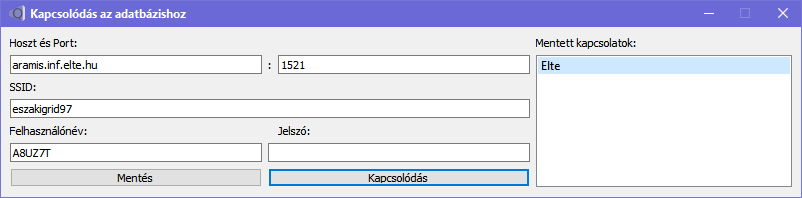
\includegraphics[width=1.0\textwidth]{Connect}
A mentett kapcsolatok kezelésére itt is lehetőség van. A \textit{delete} billentyű lenyomására a kijelölt kapcsolat törlődik.
Lehetőség van az aktuális, képernyőn látható adatok mentésére is. Ekkor egy nevet meg kell adni a kapcsolatnak, ami nem lehet üres.
Az adatok helyes megadása után, illetve ha létrejön sikeresen a kapcsolat az adatbázissal, akkor a program beléptet a szerkesztő felülethez.
Hiba esetén kiírja a hiba kódot, amivel keresse meg adatbázisának adminisztrátorát, vagy nézzen utána az Oracle oldalán.

Néhány példa a hibakódokra:
\begin{itemize}
  \item \textbf{ORA-12560}: TNS:protocol adapter error; Unable to logon. Ezt okozhatja internet kapcsolat hiánya,
  vagy hiányzó szervernév, azaz ha nem lehet kiépíteni kapcsolatot a szerverrel bármilyen okból.
  \item \textbf{ORA-01005}: null password given; logon denied; Unable to logon. Ezt a hibaüzenetet akkor kapja az ember,
  ha a jelszó mezőt üresen hagyja. (Ha üres a jelszó mező akkor hibás felhasználónév esetén is ez a hibaüzenet jön elő)
  \item \textbf{ORA-01017}: invalid username/password; logon denied; Unable to logon. Hibás felhasználónév vagy jelszó esetén.
\end{itemize}

Ezek a hibakódok természetesen más esetben is előjöhetnek, ha biztos benne hogy minden rendben van az adatokkal és a
kapcsolattal, akkor kérjen meg egy hozzáértőt a probléma elhárításában.

Az \href{https://docs.oracle.com/cd/B28359_01/server.111/b28278/toc.htm}{Oracle Docs} oldalon megtalálható minden hibakód, és annak oka (angolul). Legtöbb esetben elég beszédesek, így meg lehet őket érteni utána járás nélkül is,
persze csak angol tudás birtokában. A későbbiekben is ezen hibakódok vannak használva (és logolva), így ezt az oldalt érdemes lementeni.

\section{Grafikus felület}

\chapter{Fejlesztői dokumentáció}

\end{document}